\section{Ground State Energy and Vacuum Amplitude}
\subsection{Meaning of the vacuum amplitude}
One of the first many-body problems to be tackled by the field theoretical diagram techniques was that of finding the ground state energy $E_0$ of a system of interacting fermions. The diagrammatic methods in this chapter provide a neat way of handling nuclear and electron interactions. In both cases, we can perform a partial sum over an infinite series of infinite terms and get a finite result. In order to do this, it is necessary to have a general way of writing down the nth-order term in the ordinary perturbation series for $E_0$,i.e., in
\begin{equation}E_{0}=W_{0}+\left\langle\Phi_{0}\left|H_{1}\right| \Phi_{0}\right\rangle+\sum_{m \neq 0} \frac{\left\langle\Phi_{0}\left|H_{1}\right| \phi_{m}\right\rangle\left\langle\Phi_{m}\left|H_{1}\right| \Phi_{0}\right\rangle}{W_{0}-W_{m}}+\cdots
\label{time-indep-ground}
\end{equation}
\textbf{where $W_{0}, W_{m}$ are the ground and excited state energies of the unperturbed Hamiltonian, and $\Phi_{0}, \Phi_{m}$ are the corresponding wave functions. The general term is hard to obtain from the time-independent theory usually used to get (\ref{time-indep-ground}).} However, there is a time-dependent technique which gives a pictorial recipe for finding the desired nth-order term:\redp{\textbf{vacuum amplitude expansion.}}
\begin{imp}
The vacuum amplitude, $R(t),$ is defined as follows: Let $\Phi_{0}$ be the ground state of the unperturbed system (i.e., $\Phi_{0}$ is the \textbf{'Fermi vacuum'}). Then $R(t)$ is the probability amplitude that if the system is in $\Phi_{0}$ at time $0,$ and the external potential and/or interactions between particles are allowed to act, then the system will be in $\Phi_{0}$ at time $t .$ That is, $R(t)$ is the \textbf{\redp{'Fermi vacuum to Fermi vacuum transition amplitude'}}. $R(t)$ can also be called \textbf{"no-particle propagator"}.
\end{imp}
If there is no interaction, then the wave function at time $t$ will simply be $\Phi_0e^{-iW_0t}$ where $W_0$ is the ground state energy. If the interaction is now switched on at time $t=0$, the system will start to make transition from $\Phi_0$ to all possible N-particle states. Let the state after time $t$ be $\Psi(t)$, \bluep{\textbf{this must be obtainable fro m the ground state $\Phi_0$, by some sort of operation.}} Thus:
\begin{equation}\Psi(t)=U(t) \Phi_{0}\end{equation}
which may be regarded as the equation defining the \textbf{"time development operator"},$U(t)$. The probability amplitude $R(t)$ is thus:
\begin{imp}
\begin{equation}\begin{aligned}
R(t) &=\left(\Phi_{0} e^{-i W_{0} t}, \Psi(t)\right)=\int \Phi_{0}^{*} e^{+i W_{0} t} U(t) \Phi_{0} d \mathbf{r}_{1} \dots d \mathbf{r}_{N} \\
& \equiv\left\langle\Phi_{0}|U(t)| \Phi_{0}\right\rangle e^{+i W_{0} t}=\text { vacuum amplitude. }
\end{aligned}
\label{vac-amp-def}
\end{equation}
The importance of the vacuum amplitude lies in the fact that the ground state energy, $E_{0}$, may be obtained from it with the aid of the theorem
\begin{equation}E_{0}=W_{0}+\lim _{t \rightarrow \infty(1-i \eta)} i \frac{d}{d t} \ln R(t)
\label{ground-energy-theorem}
\end{equation}
where $\eta$ is an infinitesimal. Thus, if we can get a diagrammatic expansion of $R(t)$, then the diagram series for $E_0$ follows from \ref{ground-energy-theorem}.
\end{imp}
\begin{mybox}
The diagrammatic perturbation expansion of $R(t)$ is considerably more complicated because of the \textbf{"unlinked" diagrams (i.e. not all vertices are connected).} Lukily, the Logarithm of R turns out to be the sume over just \textbf{"linked diagrams"}. This is the famous \textbf{"linked cluster theorem"}.
\end{mybox}

\subsection{Quantum vacuum amplitude for one-particle system}
Consider the simplest situation first: a Fermi system consisting of one particle in an external potential, with non-degenerate energy levels-for example, an electron in a one-dimensional harmonic oscillator potential. Let the unperturbed Hamiltonian be
$$H_{0}=\frac{p^{2}}{2 m}+U(r)$$
with eigensolutions $\phi_k$,$\epsilon_k$. \bluep{The grpund state of the system consist of one particle in $\phi_1$ and no particles in any higher states;} in occupation number formalism this is $\Phi_0=|1_1,0_2,0_3,\ldots\rangle$. The corresponding ground state is just $W_0=\epsilon_1$. A typical excited state is one particle in $\phi_{k}$ and no particle in any other state: $\Phi_{\text {excited }}=\left|0_{1}, 0_{2}, \ldots, 1_{k}, \ldots\right\rangle .$ In particle-hole notation, the ground state is $\left.\Phi_{0}=|0\right\rangle,$ while a typical excited state consists of a hole in $\phi_{1}$ and a particle in $\phi_{k}: \Phi_{\text {exe }}=\left|1_{1}^{h}, 1_{k}^p\right\rangle .$ Note that in this one-particle system, there is only one possible hole state, e.g., $\phi_{1}$.

Suppose now a perturbation $V(\mathbf{r})$ is added to $H_{0} .$ The vacuum amplitude in that case is the probability amplitude that if the system starts in its ground state $\Phi_{0}$ at $t=0,$ and is acted upon zero or more times by $V(\mathrm{r}),$ then it will be in $\Phi_{0} e^{-iW_{0} t}$ at time $t .$ By analogy with the pinball case, $R(t)$ will be the sum of the probability amplitudes for all the different ways the system can start out in $\Phi_0$, interact with $V(\mathbf{r})$ arbitrary times and return to $\Phi_0$. \textbf{In the zeroth-order process, nothing at all happens as illustrated below:}
\begin{equation}
    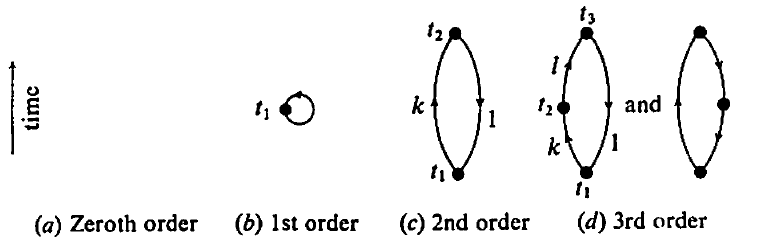
\includegraphics[width=0.8\textwidth]{screenshots/single-electron-diagram-order.PNG}
    \label{single-electron-diagram-order}
\end{equation}
In second order, at $t_1$, $V(\mathbf{t})$ can scatter the particle up into the state $\phi_k$, thus simultaneously creating a hole in $\phi_1$ and a particle in $\phi_k$, and at $t_2$ scatter the particle back into $\phi_1$. The fourth-order ones are
\begin{equation}
    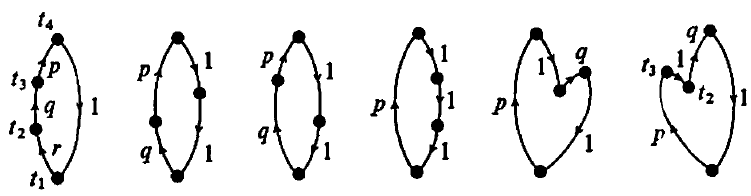
\includegraphics[width=0.8\textwidth]{screenshots/single-electron-4th-order.PNG}
    \label{single-electron-4th-order}
\end{equation}
Note that in the last two diagrams of (\ref{single-electron-4th-order}) there are two particle lines and two hole lines between $t_{2}$ and $t_{3},$ whereas our one-particle system can have at most one particle and one hole. However, it is easily shown that \textbf{these diagrams are exactly cancelled by unlinked diagrams of the sort in (\ref{single-electron-unlinked-diagram}) below}. 
\begin{equation}
    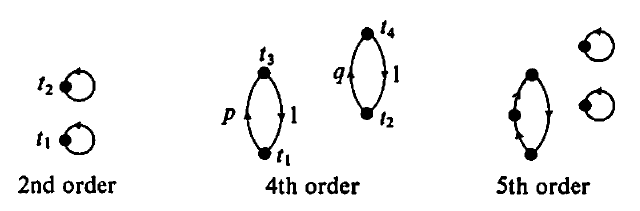
\includegraphics[width=0.8\textwidth]{screenshots/single-electron-unlinked-diagram.PNG}
    \label{single-electron-unlinked-diagram}
\end{equation}
For example, because of \textbf{the (-1) from the extra fermion loop}, the last diagram in (\ref{single-electron-4th-order}) is cancelled by the fourth-order diagram in (\ref{single-electron-unlinked-diagram}). \bluep{Nevertheless, it is necessary to retain such diagrams which violate conservation of particle number, in order to prove the linked cluster theorem.} The same argument holds for diagrams which violate the Pauli exclusion principle.

In order to draw all diagrams in $n$ th order, draw $n$ dots in a vertical row, label them $t_{1}, t_{2}, \ldots, t_{n}$ and connect them up in all possible \textbf{'topologically distinct'} (see below) ways with one line entering and one leaving each dot. For example in third order we find the six diagrams
\begin{center}
    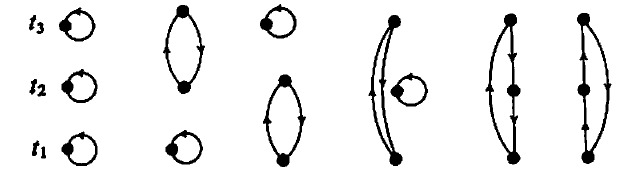
\includegraphics[width=0.8\textwidth]{screenshots/single-electron-topo-distinct.PNG}
\end{center}
Two diagrams are ' \textbf{topologically equivalent}' if one can be \bluep{distorted into the other without changing the vertical ordering of the dots; otherwise they are distinct.} This is illustrated by the fourth-order diagrams (\textbf{note significance of the direction of the arrows}).

Finally, the diagrammatic expansion for the vacuum amplitude will just be the sum of all diagrams such as the above:
\begin{equation}
    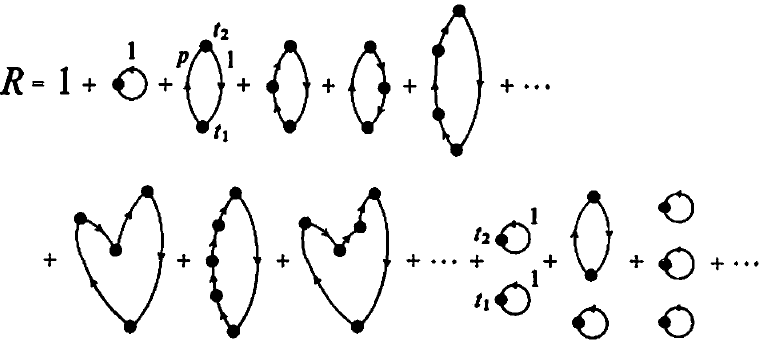
\includegraphics[width=0.8\textwidth]{screenshots/single-electron-ground-expansion.PNG}
    \label{single-electron-ground-expansion}
\end{equation}
where the 1 expresses the fact that in the unperturbed case, the probability amplitude for the system staying in its ground state is 1. Translate the series into equation we have
\begin{equation}
    \begin{aligned}
    R(t)=1-&V_{11} \int_{0}^{t} d t_{1} G_{0}\left(1, t_{1}-t_{1}\right)-\\
    &-\sum_{p>1} V_{1p} V_{p 1} \int_{0}^{t} d t_{1} \int_{0}^{t} \underset{t_2>t_1}{dt_2} G_{0}^{+}\left(p, t_{2}-t_{1}\right) G_{0}^{-}\left(1, t_{1}-t_{2}\right)+\cdots\\
    &+V_{11} V_{11} \int_{0}^{t} d t_{1} \int_{0}^{t} \underset{t_2>t_1}{d t_{2}} \quad G_{0}^{-}\left(1, t_{1}-t_{1}\right) \sigma_{0}\left(1, t_{2}-t_{2}\right)+\cdots
    \end{aligned}
\end{equation}

\subsection{Linked cluster theorem for one-particle system}